\def\pathToRoot{../../}\input{\pathToRoot headers/uebungHeader}

\DeclareMathOperator{\myIn}{in}

\usetikzlibrary{fit}
\usetikzlibrary{knots}
\usetikzlibrary{hobby}
\tikzstyle{morphism}=[draw, minimum size=0.5cm, semithick]
\tikzstyle{phantom morphism}=[minimum size=0.5cm]
\tikzstyle{object}=[semithick]
\tikzstyle{cap object}=[object, out=90, in=90, looseness=2]
\tikzstyle{cup object}=[object, out=270, in=270, looseness=2]
\tikzstyle{highlight box}=[draw, dotted]

\graphicspath{{graphics/}}


\begin{document}
\uebunghead{Talk 12}{Monoidal categories and string diagrams}
\author{Felix Rech}


\begin{exercise}
  Let $A$, $B$, $C$, $D$, be objects in a monoidal category.
  Construct a morphism
  \[
    \roundddd{\rounddd{(A \otimes I) \otimes B} \otimes C} \otimes D
    \to A \otimes \roundddd{B \otimes \rounddd{C \otimes (I \otimes D)}}.
  \]
  Can you find another?
\end{exercise}

\begin{answer}
  We construct the morphism as
  \[ \begin{tikzcd}
    (((A \otimes I) \otimes B) \otimes C) \otimes D
      \arrow[d, "((\rho_A \otimes 1_B) \otimes 1_C) \otimes 1_D"] \\
    ((A \otimes B) \otimes C) \otimes D
      \arrow[d, "\alpha_{A, B, C} \otimes 1_D"] \\
    (A \otimes (B \otimes C)) \otimes D
      \arrow[d, "\alpha_{A, B \otimes C, D}"] \\
    A \otimes ((B \otimes C) \otimes D)
      \arrow[d, "1_A \otimes \alpha_{B, C, D}"] \\
    A \otimes (B \otimes (C \otimes D))
      \arrow[d, "1_A \otimes (1_B \otimes (1_C \otimes \lambda_D^{-1}))"] \\
    A \otimes (B \otimes (C \otimes (I \otimes D))).
  \end{tikzcd} \]
  We have no more information about the category except that it is monoidal.
  In this setting we cannot construct two different morphisms of the same type, which follows from the coherence theorem.
\end{answer}


\begin{exercise}
  Convert the following algebraic equations into graphical language.
  Which would you expect to be true in any symmetric monoidal category?
  \begin{enumerate}
    \item
      $(g \otimes 1) \of \sigma \of (f \otimes 1)
        = (f \otimes 1) \of \sigma \of (g \otimes 1)$ \\
      for $A \xrightarrow{f, g} A$.

    \item
      $h \of (1 \otimes \lambda) \of (1 \otimes (f \otimes 1)) \of (1 \otimes \lambda^{-1}) \of g
        = h \of g \of \lambda \of (f \otimes 1) \of \lambda^{-1}$ \\
      for $A \xrightarrow{g} B \otimes C$, $I \xrightarrow{f} I$ and $B \otimes C \xrightarrow{h} D$.

    \item
      $\rho \of (1 \otimes f) \of \alpha \of (\sigma \otimes 1)
        = \lambda \of (f \otimes 1) \of \alpha^{-1} \of (1 \otimes \sigma) \of \alpha$ \\
      for $A \otimes B \xrightarrow{f} I$.
  \end{enumerate}
\end{exercise}

\begin{answer}
  \begin{enumerate}
  \item
    \[ \vcenter{ \hbox{ \begin{tikzpicture}
      \coordinate (in_f) at (0, 0);
      \node[morphism] (f) at (0, 1) {$f$};
      \node[phantom morphism] (f') at (1, 2.5) {};
      \coordinate (out_f) at (1, 3.5);

      \coordinate (in_g) at (1, 0);
      \node[phantom morphism] (g') at (1, 1) {};
      \node[morphism] (g) at (0, 2.5) {$g$};
      \coordinate (out_g) at (0, 3.5);

      \begin{knot}[clip width=8]
        \strand[object] (in_f)
          to node[auto] {$A$} (f.south)
          (f.north) to[out=90, in=270] (f'.south)
          to (f'.north)
          to node[auto] {$A$} (out_f);
        \strand[object] (in_g)
          to node[auto] {$A$} (g'.south)
          to (g'.north)
          to[out=90, in=270] (g.south)
          (g.north) to node[auto] {$A$} (out_g);
      \end{knot}
    \end{tikzpicture}}}
    =
    \vcenter{ \hbox{ \begin{tikzpicture}
      \coordinate (in_f) at (0, 0);
      \node[morphism] (f) at (0, 1) {$g$};
      \node[phantom morphism] (f') at (1, 2.5) {};
      \coordinate (out_f) at (1, 3.5);

      \coordinate (in_g) at (1, 0);
      \node[phantom morphism] (g') at (1, 1) {};
      \node[morphism] (g) at (0, 2.5) {$f$};
      \coordinate (out_g) at (0, 3.5);

      \begin{knot}[clip width=8]
        \strand[object] (in_f)
          to node[auto] {$A$} (f.south)
          (f.north) to[out=90, in=270] (f'.south)
          to (f'.north)
          to node[auto] {$A$} (out_f);
        \strand[object] (in_g)
          to node[auto] {$A$} (g'.south)
          to (g'.north)
          to[out=90, in=270] (g.south)
          (g.north) to node[auto] {$A$} (out_g);
      \end{knot}
    \end{tikzpicture}}} \]


  \item
    \[ \vcenter{ \hbox{ \begin{tikzpicture}
      \coordinate (in) at (0, 0);

      \node[phantom morphism] (g_left) at (-1, 1) {};
      \node[phantom morphism] (g_right) at (1, 1) {};
      \node[morphism, fit=(g_left) (g_right), inner sep=0] (g) {};
      \node at (g) {$g$};

      \node[morphism] (f) at (0, 2) {$f$};

      \node[phantom morphism] (h_left) at (-1, 3) {};
      \node[phantom morphism] (h_right) at (1, 3) {};
      \node[morphism, fit=(h_left) (h_right), inner sep=0] (h) {};
      \node at (h) {$h$};

      \coordinate (out) at (0, 4);

      \draw[object] (in) to node[auto] {$A$} (g);
      \draw[object] (-1, 0 |- g.north) to node[auto] {$B$} (-1, 0 |- h.south);
      \draw[object] (1, 0 |- g.north) to node[auto] {$C$} (1, 0 |- h.south);
      \draw[object] (h) to node[auto] {$D$} (out);
    \end{tikzpicture}}}
    =
    \vcenter{ \hbox{ \begin{tikzpicture}
      \coordinate (in) at (0, 0);

      \node[morphism] (f) at (-1, 1) {$f$};

      \node[phantom morphism] (g_left) at (-1, 2) {};
      \node[phantom morphism] (g_right) at (1, 2) {};
      \node[morphism, fit=(g_left) (g_right), inner sep=0] (g) {};
      \node at (g) {$g$};

      \node[phantom morphism] (h_left) at (-1, 3) {};
      \node[phantom morphism] (h_right) at (1, 3) {};
      \node[morphism, fit=(h_left) (h_right), inner sep=0] (h) {};
      \node at (h) {$h$};

      \coordinate (out) at (0, 4);

      \draw[object] (in) to node[auto] {$A$} (g);
      \draw[object] (-1, 0 |- g.north) to node[auto] {$B$} (-1, 0 |- h.south);
      \draw[object] (1, 0 |- g.north) to node[auto] {$C$} (1, 0 |- h.south);
      \draw[object] (h) to node[auto] {$D$} (out);
    \end{tikzpicture}}} \]

  \item
    \[ \vcenter{ \hbox{ \begin{tikzpicture}
      \coordinate (A_in) at (0, 0);
      \coordinate (C_in) at (1, 0);
      \coordinate (B_in) at (2, 0);
      \node[phantom morphism] (C_1) at (0, 1.5) {};

      \node[phantom morphism] (f_left) at (1, 1.5) {};
      \node[phantom morphism] (f_right) at (2, 1.5) {};
      \node[morphism, fit=(f_left) (f_right), inner sep=0] (f) {};
      \node at (f) {$f$};

      \coordinate (out) at (0, 2);

      \draw[object] (B_in) to node[auto, at start] {$B$} (B_in |- f.south);

      \begin{knot}[clip width=8]
        \strand[object, out=90, in=270] (A_in)
          to node[auto, at start] {$A$} (C_in |- f.south);
        \strand[object, out=90, in=270] (C_in)
          to node[auto, at start] {$C$} (C_1.south)
          to (out);
      \end{knot}
    \end{tikzpicture}}}
    =
    \vcenter{ \hbox{ \begin{tikzpicture}
      \coordinate (A_in) at (0, 0);
      \coordinate (C_in) at (1, 0);
      \coordinate (B_in) at (2, 0);
      \node[phantom morphism] (C_1) at (2, 1.5) {};

      \node[phantom morphism] (f_left) at (0, 1.5) {};
      \node[phantom morphism] (f_right) at (1, 1.5) {};
      \node[morphism, fit=(f_left) (f_right), inner sep=0] (f) {};
      \node at (f) {$f$};

      \coordinate (out) at (2, 2);

      \draw[object] (A_in) to node[auto, at start] {$A$} (A_in |- f.south);

      \begin{knot}[clip width=8]
        \strand[object, out=90, in=270] (C_in)
          to node[auto, at start] {$C$} (C_1.south)
          to (out);
        \strand[object, out=90, in=270] (B_in)
          to node[auto, at start] {$B$} (C_in |- f.south);
      \end{knot}
    \end{tikzpicture}}} \]
  \end{enumerate}

  The correctness theorem for the graphical calculus on symmetric monoidal categories tells us that two diagrams describe the same morphism if and only if they are isotopic in four-dimensional space.
  This means essentially that nodes can move accross edges and that edges can move \textit{through} each other.
  With this we can see that equations (b) and (c) hold, but not equation (a).
\end{answer}


\begin{exercise}
    Consider the following diagrams in the graphical calculus:

    \centering 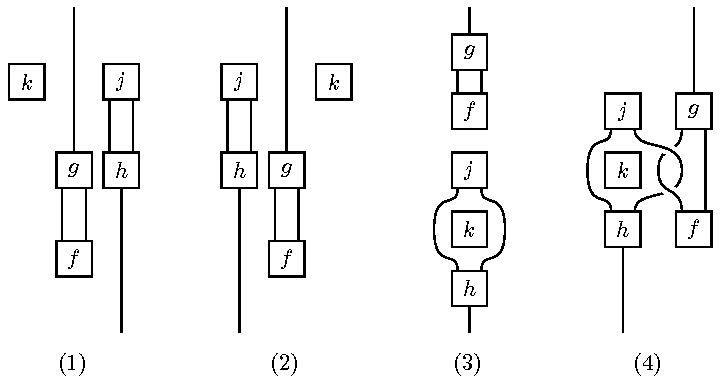
\includegraphics{monoidal-braided-symmetric-comparison}

    \begin{enumerate}
      \item Which diagrams are equal as morphisms in a monoidal category?
      \item Which diagrams are equal as morphisms in a braided monoidal category?
      \item Which diagrams are equal as morphisms in a symmetric monoidal category?
    \end{enumerate}
\end{exercise}

\begin{answer}
  \begin{enumerate}
  \item
    We regard the diagrams up to planar isotopy.
    Thus diagrams (1) and (2) are equal but (3) and (4) are not equal to any other diagram.
  \item
    We regard the diagrams up to spacial isotopy.
    Thus diagrams (1), (2) and (3) are equal but (4) is not equal to any other diagram.
  \item
    We regard the diagrams up to four-dimensional isotopy.
    Thus all diagrams are equal.
  \end{enumerate}
\end{answer}

\ifdefined\issolution \else \pagebreak \fi
\begin{exercise}
  Verify the correctness of the following graphical equations in braided monoidal categories by
  \begin{enumerate}
    \item the correctness theorem of the graphical calculus,
    \item substitution in string diagrams using the axioms of braided monoidal categories and the correctness theorem for the graphical calculus on general monoidal categories,
    \item construction of a commuting diagram from the axioms and the coherence theorem for general monoidal categories.
  \end{enumerate}
  \begin{enumerate}[label=(\roman*)]
    \item $\vcenter{\hbox{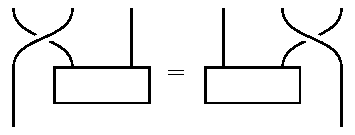
\includegraphics{proofs_by_hand_1}}}$
    \item $\vcenter{\hbox{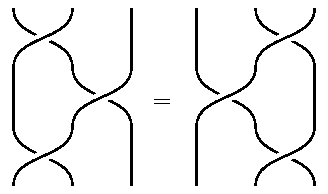
\includegraphics{proofs_by_hand_2}}}$
    \item $\vcenter{\hbox{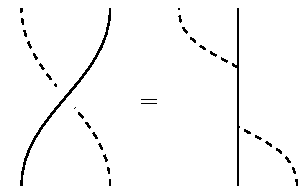
\includegraphics{proofs_by_hand_3}}}$
      ($\sigma_{A, I} = \lambda_{A}^{-1} \of \rho_A$)
  \end{enumerate}
\end{exercise}

\begin{answer}
  \begin{enumerate}
  \item
    In three-dimensional space, the diagrams are obviously isotopic.
    The equations follow directly from the correctness theorem.
  \item
    \begin{enumerate}
    \item
      \[
        \vcenter{ \hbox{ \begin{tikzpicture}
          \node[phantom morphism] (in) at (0, -0.5) {};
          \node[phantom morphism] (f_left) at (1, 2) {};
          \node[phantom morphism] (f_right) at (2, 2) {};
          \node[morphism, fit=(f_left) (f_right), inner sep=0] (f) {};
          \node[phantom morphism] (out_1) at (0, 4) {};
          \node[phantom morphism] (out_2) at (1, 4) {};
          \node[phantom morphism] (out_3) at (2, 4) {};

          \begin{knot}[clip width=8]
            \strand[object, out=90, in=270] (in)
              to (in |- f.north)
              to (out_2);
            \strand[object, out=90, in=270] (f_left) to (out_1);
            \strand[object, out=90, in=270] (f_right) to (out_3);
          \end{knot}
        \end{tikzpicture} } }
        =
        \vcenter{ \hbox{ \begin{tikzpicture}[use Hobby shortcut]
          \node[phantom morphism] (in) at (2.5, -0.5) {};
          \node[phantom morphism] (f_left) at (0.5, 1) {};
          \node[phantom morphism] (f_right) at (1.5, 1) {};
          \node[morphism, fit=(f_left) (f_right), inner sep=0] (f) {};
          \node[phantom morphism] (out_1) at (1, 4) {};
          \node[phantom morphism] (out_2) at (2, 4) {};
          \node[phantom morphism] (out_3) at (3, 4) {};

          \begin{knot}[clip width=8]
            \strand[object, out=90, in=270] (in)
              to (in |- f.north)
              to (1, 2.5)
              to (out_2);
            \strand[object, in angle=-90, out angle=90, in=-90, out=90] (f_left.north)
              .. (1.6, 1.92)
              .. (out_2 |- 0, 2.5)
              to (out_1);
            \strand[object, in angle=-90, out angle=90, in=-90, out=90]
              (f_right.north)
              .. (1.9, 1.83)
              .. (out_3 |- 0, 2.5)
              to (out_3);
          \end{knot}
        \end{tikzpicture} } }
        =
        \vcenter{ \hbox{ \begin{tikzpicture}
          \node[phantom morphism] (in) at (2, 0) {};
          \node[phantom morphism] (f_left) at (0, 1) {};
          \node[phantom morphism] (f_right) at (1, 1) {};
          \node[morphism, fit=(f_left) (f_right), inner sep=0] (f) {};
          \node[phantom morphism] (out_1) at (0, 4.5) {};
          \node[phantom morphism] (out_2) at (1, 4.5) {};
          \node[phantom morphism] (out_3) at (2, 4.5) {};

          \begin{knot}[clip width=8]
            \strand[object, out=90, in=270] (in)
              to (in |- f.north)
              to (0, 3)
              to (out_2);
            \strand[object, in=-90, out=90] (f_left.north)
              to (0, 2)
              to (1, 3)
              to (out_1);
            \strand[object, in=-90, out=90]
              (f_right.north)
              to (2, 2.5)
              to (out_3);
          \end{knot}
        \end{tikzpicture} } }
        =
        \vcenter{ \hbox{ \begin{tikzpicture}
          \node[phantom morphism] (in) at (2, 0) {};
          \node[phantom morphism] (f_left) at (0, 1) {};
          \node[phantom morphism] (f_right) at (1, 1) {};
          \node[morphism, fit=(f_left) (f_right), inner sep=0] (f) {};
          \node[phantom morphism] (out_1) at (0, 4.5) {};
          \node[phantom morphism] (out_2) at (1, 4.5) {};
          \node[phantom morphism] (out_3) at (2, 4.5) {};

          \begin{knot}[clip width=8]
            \strand[object, out=90, in=270] (in)
              to (in |- f.north)
              to (1, 2.5)
              to (out_2);
            \strand[object, out=90, in=270] (f_left) to (out_1);
            \strand[object, out=90, in=270] (f_right) to (2, 2.5) to (out_3);
          \end{knot}
        \end{tikzpicture} } }
      \]
      In step one we apply naturality of $\sigma^{-1}$, in step two we apply one hexagon equality and in step three we cancel inverses.
      Note that we implicitly use the equality from (iii) to justify that we cross the invisible unit object below the box with another object in step one.

    \item
      \[
        \vcenter{ \hbox{ \begin{tikzpicture}
          \begin{knot}[clip width=8]
            \strand[object, in=-90, out=90]
              (0, 0)
              to (1, 1)
              to (2, 2)
              to (2, 3);
            \strand[object, in=-90, out=90]
              (1, 0)
              to (0, 1)
              to (0, 2)
              to (1, 3);
            \strand[object, in=-90, out=90]
              (2, 0)
              to (2, 1)
              to (1, 2)
              to (0, 3);
          \end{knot}

          % \draw[highlight box] (-0.2, 0) rectangle (2.2, 2);
        \end{tikzpicture} } }
        =
        \vcenter{ \hbox{ \begin{tikzpicture}[use Hobby shortcut]
          \begin{knot}[clip width=8]
            \strand[object, in=-90, out=90]
              (0, 0)
              to (2, 2)
              to (2, 3);
            \strand[object, in angle=-90, out angle=90, in=-90, out=90]
              (1, 0)
              .. (0.9, 1)
              .. (0, 2)
              to (1, 3);
            \strand[object, in angle=-90, out angle=90, in=-90, out=90]
              (2, 0)
              .. (1.1, 1)
              .. (1, 2)
              to (0, 3);
          \end{knot}
        \end{tikzpicture} } }
        =
        \vcenter{ \hbox{ \begin{tikzpicture}[use Hobby shortcut]
          \begin{knot}[clip width=8]
            \strand[object, in=-90, out=90]
              (0, 0)
              to (0, 1)
              to (2, 3);
            \strand[object, in angle=-90, out angle=90, in=-90, out=90]
              (1, 0)
              to (2, 1)
              .. (1.1, 2)
              .. (1, 3);
            \strand[object, in angle=-90, out angle=90, in=-90, out=90]
              (2, 0)
              to (1, 1)
              .. (0.9, 2)
              .. (0, 3);
          \end{knot}

          % \draw[highlight box] (-0.2, 1) rectangle (2.2, 3);
        \end{tikzpicture} } }
        =
        \vcenter{ \hbox{ \begin{tikzpicture}
          \begin{knot}[clip width=8]
            \strand[object, in=-90, out=90]
              (0, 0)
              to (0, 1)
              to (1, 2)
              to (2, 3);
            \strand[object, in=-90, out=90]
              (1, 0)
              to (2, 1)
              to (2, 2)
              to (1, 3);
            \strand[object, in=-90, out=90]
              (2, 0)
              to (1, 1)
              to (0, 2)
              to (0, 3);
          \end{knot}
        \end{tikzpicture} } }
      \]
      We apply one hexagon equality in step one, naturality of $\sigma$ in step two and the other hexagon equality in step three.

    \item
      \[
        \vcenter{ \hbox{ \begin{tikzpicture}[x=0.75cm]
          \begin{knot}[clip width=8]
            \strand[object, in=-90, out=90] (-1, 0) to (1, 4.5);
            \strand[object, dashed, in=-90, out=90] (1, 0) to (-1, 4.5);
          \end{knot}
        \end{tikzpicture} } }
        =
        \vcenter{ \hbox{ \begin{tikzpicture}[x=0.75cm]
          \begin{knot}[clip width=8]
            \strand[object, in=-90, out=90]
              (0, 0)
              to (0, 4.5);
            \strand[object, dashed, in=-90, out=90]
              (1, 0)
              to (-1, 1.5)
              to (1, 3)
              to (-1, 4.5);
          \end{knot}
        \end{tikzpicture} } }
        =
        \vcenter{ \hbox{ \begin{tikzpicture}[x=0.75cm]
          \begin{knot}[clip width=8]
            \strand[object, in=-90, out=90]
              (0, 0)
              to (0, 4.5);
            \strand[object, dashed, in=-90, out=90]
              (1, 0)
              to (-1, 1.4)
              to (-1, 1.6)
              to (1, 3.1)
              (-1, 1.4)
              to (1, 2.9)
              to (1, 3.1)
              to (-1, 4.5);
          \end{knot}
        \end{tikzpicture} } }
        =
        \vcenter{ \hbox{ \begin{tikzpicture}[x=0.75cm]
          \begin{knot}[clip width=8]
            \strand[object, in=-90, out=90]
              (0, 0)
              to (0, 4.5);
            \strand[object, dashed, in=-90, out=90]
              (1, 0)
              to (-1, 1)
              to (-1, 2)
              to (1, 3.5)
              (-1, 1)
              to (1, 2.5)
              to (1, 3.5)
              to (-1, 4.5);
          \end{knot}
        \end{tikzpicture} } }
        =
        \vcenter{ \hbox{ \begin{tikzpicture}[x=0.75cm]
          \begin{knot}[clip width=8]
            \strand[object]
              (0, 0)
              to (0, 4.5);
            \strand[object, dashed, dashed, in=-90, out=90]
              (1, 0)
              to (-1, 1)
              to (1, 2)
              to[in=0] (0, 2.5)
              (0, 2)
              to[out=180] (-1, 2.5)
              to (1, 3.5)
              to (-1, 4.5);
          \end{knot}
        \end{tikzpicture} } }
        =
        \vcenter{ \hbox{ \begin{tikzpicture}[x=0.75cm]
          \begin{knot}[clip width=8]
            \strand[object]
              (0, 0)
              to (0, 4.5);
            \strand[object, dashed, in=-90, out=90]
              (1, 0)
              to[in=-45] (0, 3)
              (0, 1.5)
              to[out=135] (-1, 4.5);
          \end{knot}
        \end{tikzpicture} } }
        =
        \vcenter{ \hbox{ \begin{tikzpicture}[x=0.75cm]
          \begin{knot}[clip width=8]
            \strand[object]
              (0, 0)
              to (0, 4.5);
            \strand[object, dashed, in=-90, out=90]
              (1, 0)
              to[in=-45] (0, 1.5)
              (0, 3)
              to[out=135] (-1, 4.5);
          \end{knot}
        \end{tikzpicture} } }
      \]
      We introduce $\sigma$ with it's inverse in step one.
      We apply naturality of $\sigma^{-1}$ in step two and one hexagon equation in step three.
      The rest follows from the naturality of $\lambda$ and $\rho$ with the correctness of the graphical calculus for general monoidal categories and cancellation of inverses.
    \end{enumerate}
  \item
    \begin{enumerate}
    \item
      \[ \begin{tikzcd}[column sep=0.5cm]
        & B
          \arrow[ld, "\rho_B^{-1}"']
          \arrow[rd, "\lambda_B^{-1}"] \\
        %
        B \otimes I
          \arrow[rr, "\sigma_{B, I}"]
          \arrow[d, "1_B \otimes f"] &&
        I \otimes B
          \arrow[d, "f \otimes 1_B"] \\
        %
        B \otimes (A \otimes C)
          \arrow[rr, "\sigma_{B, A \otimes C}"]
          \arrow[d, "\alpha_{B, A, C}^{-1}"] &&
        (A \otimes C) \otimes B
          \arrow[d, "\alpha_{A, C, B}"] \\
        %
        (B \otimes A) \otimes C
          \arrow[d, "\sigma_{B, A} \otimes 1_C"] &&
        A \otimes (C \otimes B)
          \arrow[d, "1_A \otimes \sigma_{C, B}"] \\
        %
        (A \otimes B) \otimes C
          \arrow[rr, "\alpha_{A, B, C}"] &&
        A \otimes (B \otimes C)
      \end{tikzcd} \]
      The left outer path describes the first diagram and the right outer path describes the second diagram.
      From top to bottom, the parts commute by the equality from (iii), naturality of $\sigma$ and one hexagon equality.

    \item
      \[ \begin{tikzcd}[column sep=1.2cm]
        (A \otimes B) \otimes C
          \arrow[r, "\alpha_{A, B, C}"]
          \arrow[d, "\sigma_{A, B} \otimes 1_C"] &
        A \otimes (B \otimes C)
          \arrow[d, "1_A \otimes \sigma_{B, C}"] \\
        %
        (B \otimes A) \otimes C
          \arrow[d, "\alpha_{B, A, C}"] &
        A \otimes (C \otimes B)
          \arrow[d, "\alpha_{A, C, B}^{-1}"] \\
        %
        B \otimes (A \otimes C)
          \arrow[r, "\sigma_{B, A \otimes C}"]
          \arrow[d, "1_B \otimes \sigma_{A, C}"] &
        (A \otimes C) \otimes B
          \arrow[d, "\sigma_{A, C} \otimes 1_B"] \\
        %
        B \otimes (C \otimes A)
          \arrow[r, "\sigma_{B, C \otimes A}"]
          \arrow[d, "\alpha_{B, C, A}^{-1}"] &
        (C \otimes A) \otimes B
          \arrow[d, "\alpha_{C, A, B}"] \\
        %
        (B \otimes C) \otimes A
          \arrow[d, "\sigma_{B, C} \otimes 1_A"] &
        C \otimes (A \otimes B)
          \arrow[d, "1_C \otimes \sigma_{A, B}"] \\
        %
        (C \otimes B) \otimes A
          \arrow[r, "\alpha_{C, B, A}"] &
        C \otimes (B \otimes A)
      \end{tikzcd} \]
      The left outer path describes the first diagram and the right outer path describes the second diagram.
      The parts of the diagram commute by the hexagon equalities and naturality of $\sigma$.

    \item
      \[ \begin{tikzcd}
        I \otimes A
          \arrow[rrrrrr, bend left, "\sigma"]
          \arrow[r, "\sigma"]
          \arrow[rrdd, "\rho^{-1}"']
          \arrow[rrrddd, bend right, "\lambda"'] &
        A \otimes I
          \arrow[rrrr, bend left, "\sigma"]
          \arrow[r, "1 \otimes \lambda^{-1}"]
          \arrow[rd, "\rho^{-1}"'] &
        A \otimes (I \otimes I)
          \arrow[rr, "\sigma"]
          \arrow[d, "\alpha^{-1}"] &&
        (I \otimes I) \otimes A
          \arrow[d, "\alpha"'] &
        I \otimes A
          \arrow[l, "\lambda^{-1} \otimes 1"']
          \arrow[ld, "\lambda^{-1}"] &
        A \otimes I
          \arrow[l, "\sigma"']
          \arrow[lldd, "\lambda^{-1}"]
          \arrow[lllddd, bend left, "\rho"] \\
        %
        && (A \otimes I) \otimes I
          \arrow[d, "\sigma \otimes 1"] &&
        I \otimes (I \otimes A)
          \arrow[d, "1 \otimes \sigma"'] \\
        %
        && (I \otimes A) \otimes I
          \arrow[rr, "\alpha"] &&
        I \otimes (A \otimes I) \\
        %
        &&& A
      \end{tikzcd} \]
      The rectangle in the middle represents one hexagon equality.
      The section above it commutes by naturality of $\sigma$.
      The squares to its right and left commute by naturality of $\lambda$ and $\rho$.
      Everything else commutes trivially or by the coherence theorem for general monoidal categories.
    \end{enumerate}
  \end{enumerate}
\end{answer}


\begin{exercise}
  Show that $\Set$ is a symmetric monoidal category under $I \coloneqq \emptyset$ and $A \otimes B \coloneqq A + B + (A \times B)$, where we write $\times$ for Cartesian product of sets and $+$ for disjoint union of sets.
\end{exercise}

\begin{answer}
  First we show that this describes a monoidal category.
  The tensor product an unit are already given.
  The next step is to define the associator and unitors.
  We ignore some parentheses in our notation and denote by $\myIn_i : A_i \to A_1 + \cdots + A_i + \cdots + A_n$ the injection into the $n$-ary disjoint union for all families of sets $A_1, \ldots, A_n$ and indices $1 \leq i \leq n$.
  We define the associator and unitors by pattern matching:
  \begin{align*}
    \alpha_{A, B, C} &: A + B + (A \times B) + C + \roundddd{\rounddd{A + B + (A \times B)} \times C} \\
      &\qquad \to A + B + C + (B \times C) + \roundddd{A \times \rounddd{B + C + (B \times C)}} \\
    \alpha(\myIn_1(a)) &= \myIn_1(a) \\
    \alpha(\myIn_2(b)) &= \myIn_2(b) \\
    \alpha(\myIn_3(a, b)) &= \myIn_5(a, \myIn_1(b)) \\
    \alpha(\myIn_4(c)) &= \myIn_3(c) \\
    \alpha(\myIn_5(\myIn_1(a), c)) &= \myIn_5(a, \myIn_2(c)) \\
    \alpha(\myIn_5(\myIn_2(b), c)) &= \myIn_4(b, c) \\
    \alpha(\myIn_5(\myIn_3(a, b), c)) &= \myIn_5(a, \myIn_3(b, c)) \\
    \\
    \lambda_{A} &: \emptyset + A + (\emptyset \times A) \to A \\
    \lambda(\myIn_2(a)) &= a \\
    \\
    \rho_{A} &: A + \emptyset + (A \times \emptyset) \to A \\
    \rho(\myIn_1(a)) &= a.
  \end{align*}
  Those are obviously bijections since you can basically swap the terms on both sides of the defining equations and get the definition of the inverse.
  They describe natural transformations because they do not change the elements of $A$, $B$ and $C$ but only repackage them.
  To check the triangle and pentagon equalities, is trivial but tedious because you have to make many case distinctions.
  It is best done with a proof assistant.
  We omit it here.

  We showed that $\emptyset$ and $\otimes$ define a monoidal structure.
  Now we will show that it is even symmetric.
  We define the symmetry as
  \begin{align*}
    \sigma_{A, B} &: A + B + (A \times B) \\
      &\qquad\to B + A + (B \times A) \\
    \sigma(\myIn_1(a)) &= \myIn_2(a) \\
    \sigma(\myIn_2(b)) &= \myIn_1(b) \\
    \sigma(\myIn_3(a, b)) &= \myIn3(b, a).
  \end{align*}
  The symmetry is self-inverse because as above, we can swap the argument pattern with the right side of each defining equation and get the same set of equations back.
  Also as above, the symmetry is natural because it does not modify elements of $A$ or $B$.
  The hexagon equalities are again trivial to show, but the proof needs many case distinctions and is thus omitted here.

  Another approach is to look at a category that includes $\Set$ as subcategory but makes the symmetric monoidal structure more obvious.
  We observe that $I$ and $\otimes$ coincide with the terminal object and the product functor from the category of sets with partial functions.
  Liker every terminal object and product, they give rise to a symmetric monoidal structure.
  Since the associator, unitors and symmetry are isomorphisms, they are total and contained in $\Set$.
  Thus the symmetric monoidal structure exists also in $\Set$.
\end{answer}


\begin{exercise}
  Assume that we have morphisms $I \xrightarrow{\eta} R \otimes L$ and $L \otimes R \xrightarrow{\varepsilon, \varepsilon'} I$ in a monoidal category such that $\eta$ and $\varepsilon$ satisfy one snake equation and $\eta$ and $\varepsilon'$ satisfy the other snake equation.
  Show that this already implies $\varepsilon = \varepsilon'$.
\end{exercise}

\begin{answer}
  \[
    \vcenter{ \hbox{ \begin{tikzpicture}
      \node[phantom morphism] (epsilon_left) at (0, 1) {};
      \node[phantom morphism] (epsilon_right) at (1, 1) {};
      \node[morphism, fit=(epsilon_left) (epsilon_right), inner sep=0] (epsilon) {};
      \node at (epsilon) {$\varepsilon$};

      \coordinate (in1) at (0, -0.5);
      \coordinate (in2) at (1, -0.5);
      \draw[object] (in1) to (epsilon_left);
      \draw[object] (in2) to (epsilon_right);
    \end{tikzpicture} } }
    =
    \vcenter{ \hbox{ \begin{tikzpicture}
      \node[phantom morphism] (epsilon_left) at (0, 1) {};
      \node[phantom morphism] (epsilon_right) at (1, 1) {};
      \node[morphism, fit=(epsilon_left) (epsilon_right), inner sep=0] (epsilon) {};
      \node at (epsilon) {$\varepsilon$};

      \node[phantom morphism] (eta_left) at (1, 0) {};
      \node[phantom morphism] (eta_right) at (2, 0) {};
      \node[morphism, fit=(eta_left) (eta_right), inner sep=0] (eta) {};
      \node at (eta) {$\eta$};

      \node[phantom morphism] (epsilon'_left) at (2, 1) {};
      \node[phantom morphism] (epsilon'_right) at (3, 1) {};
      \node[morphism, fit=(epsilon'_left) (epsilon'_right), inner sep=0] (epsilon') {};
      \node at (epsilon') {$\varepsilon'$};

      \coordinate (in1) at (0, -0.5);
      \coordinate (in2) at (3, -0.5);
      \draw[object] (in1) to (epsilon_left);
      \draw[object] (eta_left) to (epsilon_right);
      \draw[object] (eta_right) to (epsilon'_left);
      \draw[object] (in2) to (epsilon'_right);
    \end{tikzpicture} } }
    =
    \vcenter{ \hbox{ \begin{tikzpicture}
      \node[phantom morphism] (epsilon'_left) at (2, 1) {};
      \node[phantom morphism] (epsilon'_right) at (3, 1) {};
      \node[morphism, fit=(epsilon'_left) (epsilon'_right), inner sep=0] (epsilon') {};
      \node at (epsilon') {$\varepsilon'$};

      \coordinate (in1) at (2, -0.5);
      \coordinate (in2) at (3, -0.5);
      \draw[object] (in1) to (epsilon'_left);
      \draw[object] (in2) to (epsilon'_right);
    \end{tikzpicture} } }
  \]
  In the first step we apply the snake equation for $\varepsilon$ and in the second step the snake equation for $\varepsilon'$.
\end{answer}


\begin{exercise}
  In a monoidal category, show that
  \begin{enumerate}
    \item if an initial object $0$ exists and $L \dashv R$, then $L \otimes 0 \iso 0 \iso 0 \otimes R$;
    \item if a terminal object $1$ exists and $L \dashv R$, then $R \otimes 1 \iso 1 \iso 1 \otimes L$.
  \end{enumerate}
\end{exercise}

\begin{answer}
  We only show the equivalence $L \otimes 0 \iso 0$.
  The other equivalences are analogous.

  We define functions in both directions by
  \[ \begin{tikzpicture}
    \node[phantom morphism] (f_left) at (1, 1) {};
    \node[phantom morphism] (f_right) at (2, 1) {};
    \node[morphism, fit=(f_left) (f_right), inner sep=0] (f) {};
    \node at (f) {$0_{R \otimes 0}$};

    \node[phantom morphism] (L_mid) at (0, 1) {};

    \coordinate (in_L) at (0, 0);
    \coordinate (in_0) at (1.5, 0);
    \coordinate (out) at (2, 2);

    \draw[object] (in_L)
      to node[auto] {$L$} (L_mid.south)
      to (L_mid.north)
      to[cap object] (f_left);
    \path (f_left) to node[auto, swap] {$R$} (f_left |- out);
    \draw[object] (in_0) to node[auto] {$0$} (f);
    \draw[object] (f_right) to node[auto, swap] {$0$} (out);
  \end{tikzpicture} \]
  and
  \[ \begin{tikzpicture}
    \node[phantom morphism] (f_left) at (0, 0) {};
    \node[phantom morphism] (f_right) at (1, 0) {};
    \node[morphism, fit=(f_left) (f_right), inner sep=0] (f) {};
    \node at (f) {$0_{L \otimes R}$};

    \draw[object] (0.5, -1) to node[auto] {$0$} (f);
    \draw[object] (f_left) to node[auto] {$L$}  (0, 1);
    \draw[object] (f_right) to node[auto] {$0$}  (1, 1);
  \end{tikzpicture}. \]
  Where $0_{R \otimes 0}$ and $0_{L \otimes 0}$ stand for the unique morphisms from the initial object.
  In one direction they are trivially inverse because morphisms from $0$ are unique.
  In the other direction it follows by
  \[
    \vcenter{ \hbox{ \begin{tikzpicture}
      \node[phantom morphism] (f_left) at (1, 1) {};
      \node[phantom morphism] (f_right) at (2, 1) {};
      \node[morphism, fit=(f_left) (f_right), inner sep=0] (f) {};
      \node at (f) {$0_{R \otimes 0}$};

      \node[phantom morphism] (g_left) at (1.5, 2) {};
      \node[phantom morphism] (g_right) at (2.5, 2) {};
      \node[morphism, fit=(g_left) (g_right), inner sep=0] (g) {};
      \node at (g) {$0_{L \otimes 0}$};

      \node[phantom morphism] (L_mid) at (0, 1) {};

      \coordinate (in_L) at (0, 0);
      \coordinate (in_0) at (1.5, 0);
      \coordinate (out_L) at (1.5, 3);
      \coordinate (out_0) at (2.5, 3);

      \draw[object] (in_L)
        to node[auto] {$L$} (L_mid.south)
        to (L_mid.north)
        to[cap object] (f_left);
      \path (f_left) to node[auto, swap] {$R$} (f_left |- g.south);
      \draw[object] (in_0) to node[auto] {$0$} (f);
      \draw[object] (f_right) to node[auto, swap] {$0$} (g);
      \draw[object] (g_left) to node[auto] {$L$} (out_L);
      \draw[object] (g_right) to node[auto] {$0$} (out_0);
    \end{tikzpicture} } }
    =
    \vcenter{ \hbox{ \begin{tikzpicture}
      \node[phantom morphism] (f_left) at (1, 1) {};
      \node[phantom morphism] (f_right) at (2.5, 1) {};
      \node[morphism, fit=(f_left) (f_right), inner sep=0] (f) {};
      \node at (f) {$0_{R \otimes 0}$};

      \node[phantom morphism] (g_left) at (2, 2) {};
      \node[phantom morphism] (g_right) at (3, 2) {};
      \node[morphism, fit=(g_left) (g_right), inner sep=0] (g) {};
      \node at (g) {$0_{L \otimes 0}$};

      \node[phantom morphism] (L_mid_1) at (0, 1) {};
      \node[phantom morphism] (L_mid_2) at (0, 2) {};
      \node[phantom morphism] (R_mid) at (1, 2) {};

      \coordinate (in_L) at (0, 0);
      \coordinate (in_0) at (1.75, 0);
      \coordinate (out_L) at (2, 3);
      \coordinate (out_0) at (3, 3);

      \draw[object] (in_L)
        to node[auto] {$L$} (L_mid_1.south)
        to (L_mid_2.north)
        to[cap object] (R_mid)
        to (f_left);
      \path (R_mid) to node[auto, swap] {$R$} (R_mid |- out_L);
      \draw[object] (in_0) to node[auto] {$0$} (f);
      \draw[object] (f_right) to node[auto] {$0$} (g);
      \draw[object] (g_left) to node[auto, swap] {$L$} (out_L);
      \draw[object] (g_right) to node[auto, swap] {$0$} (out_0);

      \node[highlight box, fit=(f) (g)] {};
    \end{tikzpicture} } }
    =
    \vcenter{ \hbox{ \begin{tikzpicture}
      \node[phantom morphism] (f_left) at (1, 1) {};
      \node[phantom morphism] (f_right) at (2.5, 1) {};
      \node[phantom morphism, fit=(f_left) (f_right), inner sep=0] (f) {};

      \node[phantom morphism] (g_left) at (2, 2) {};
      \node[phantom morphism] (g_right) at (3, 2) {};
      \node[phantom morphism, fit=(g_left) (g_right), inner sep=0] (g) {};

      \node[phantom morphism] (L_mid_1) at (0, 1) {};
      \node[phantom morphism] (L_mid_2) at (0, 2) {};
      \node[phantom morphism] (R_mid) at (1, 2) {};
      \node[phantom morphism] (L_mid_3) at (2, 2) {};

      \coordinate (in_L) at (0, 0);
      \coordinate (in_0) at (3, 0);
      \coordinate (out_L) at (2, 3);
      \coordinate (out_0) at (3, 3);

      \draw[object] (in_L)
        to node[auto] {$L$} (L_mid_1.south)
        to (L_mid_2.south)
        to (L_mid_2.north)
        to[cap object] (R_mid)
        to (R_mid.south)
        to[cup object] (L_mid_3)
        to (L_mid_3.north)
        to node[auto, swap] {$L$} (out_L);
      \path (R_mid) to node[auto, swap] {$R$} (R_mid |- out_L);
      \draw[object] (in_0)
        to node[auto] {$0$} (in_0 |- f.south)
        to (out_0 |- g.south)
        to (out_0 |- g.north)
        to node[auto, swap] {$0$} (out_0);

      \node[highlight box, fit=(f_left) (g_right)] {};
    \end{tikzpicture} } }
    =
    \vcenter{ \hbox{ \begin{tikzpicture}
      \node[phantom morphism] (L_mid) at (0, 1) {};
      \node[phantom morphism] (0_mid) at (1, 1) {};

      \draw[object] (0, 0)
        to node[auto] {$L$} (L_mid.south)
        to (0, 3);
      \draw[object] (1, 0)
        to node[auto] {$0$} (0_mid.south)
        to (1, 3);
    \end{tikzpicture} } }.
  \]
  In the second step we use again that morphisms from $0$ are unique.
\end{answer}


\begin{definition}{Idempotent, splitting}
  An endomorphism $A \xrightarrow{f} A$ is called \demph{idempotent} when $f \of f = f$. An idempotent $A \xrightarrow{f} A$ \demph{splits} when there exists an object $B$ and morphisms $A \xrightarrow{g} B$ and $B \xrightarrow{h} A$ such that $f = h \of g$ and $g \of h = 1$.
\end{definition}


\begin{exercise}
  Show that in a monoidal category where all idempotents split, if there are morphisms $I \xrightarrow{\eta} R \otimes L$ and $L \otimes R \xrightarrow{\varepsilon} I$ satisfying the first snake equation, then $L$ has a right dual (not necessarily given by $R$ with $\eta$ and $\varepsilon$).
\end{exercise}

\begin{answer}
  For clarity, we draw $\eta$ as
  \[ \begin{tikzpicture}
    \draw[object] (0, 0.5)
      to node[auto, swap] {$R$} (0, 0)
      to[cup object] (1, 0)
      to node[auto] {$L$} (1, 0.5);
    \end{tikzpicture} \]
    and $\varepsilon$ as
    \[ \begin{tikzpicture}
      \draw[object] (0, -0.5)
        to node[auto] {$L$} (0, 0)
        to[cap object] (1, 0)
        to node[auto, swap] {$R$} (1, -0.5);
    \end{tikzpicture}. \]

    Assume that we have the snake equality
    \[ \vcenter{ \hbox{ \begin{tikzpicture}
      \draw[object] (2, 2)
        to (2, 1)
        to[cup object] (1, 1)
        to[cap object] (0, 1)
        to (0, 0);
    \end{tikzpicture} } }
    =
    \vcenter{ \hbox{ \begin{tikzpicture}
      \draw (0, 2) (0, 0);
    \end{tikzpicture} } }. \]

    Then the other snake is idempotent by
    \[ \vcenter{ \hbox{ \begin{tikzpicture}
      \draw[object] (4, -1)
        to node[auto, near start] {$R$} (4, 0)
        to[cap object] (3, 0)
        to[cup object] (2, 0)
        to (2, 2)
        to[cap object] (1, 2)
        to[cup object] (0, 2)
        to node[auto, near end] {$R$} (0, 3);
    \end{tikzpicture} } }
    =
    \vcenter{ \hbox{ \begin{tikzpicture}
      \draw[object] (4, -1)
        to node[auto, very near start] {$R$} (4, 2)
        to[cap object] (3, 2)
        to (3, 1)
        { [local bounding box=inner snake]
          node[phantom morphism] {}
          to[cup object] (2, 1)
          to[cap object] (1, 1)
          node[phantom morphism] {}
        }
        to (1, 0)
        to[cup object] (0, 0)
        to node[auto, very near end] {$R$} (0, 3);
      \node[highlight box, fit=(inner snake)] {};
    \end{tikzpicture} } }
    =
    \vcenter{ \hbox{ \begin{tikzpicture}
      \draw[object] (2, -1)
        to node[auto, very near start] {$R$} (2, 2)
        to[cap object] (1, 2)
        to (1, 1)
        { [local bounding box=inner snake 2]
          node[phantom morphism] {}
        }
        to (1, 0)
        to[cup object] (0, 0)
        to node[auto, very near end] {$R$} (0, 3);
      % \node[highlight box, fit=(inner snake 2) (inner snake 2 |- inner snake.north) (inner snake 2 |- inner snake.south)] {};
    \end{tikzpicture} } }.
  \]
  Since all idempotents split, there are morphisms $R \xrightarrow{g} X$ and $ X\xrightarrow{h} R$ such that
  \[
    \vcenter{ \hbox{ \begin{tikzpicture}
      \node[phantom morphism, overlay] (out) at (0, 3) {};
      \node[morphism] (g) at (0, 2) {$g$};
      \node[morphism] (h) at (0, 1) {$h$};
      \node[phantom morphism, overlay] (in) at (0, 0) {};
      \draw[object] (in)
        to node[auto] {$X$} (h)
        to (g)
        to node[auto] {$X$} (out);
    \end{tikzpicture} } }
    =
    \vcenter{ \hbox{ \begin{tikzpicture}
      \node[phantom morphism, overlay] (out) at (0, 3) {};
      \node[phantom morphism, overlay] (in) at (0, 0) {};
      \draw[object] (in) to node[auto, very near start] {$X$} (out);
    \end{tikzpicture} } }
  \]
  and
  \[
    \vcenter{ \hbox{ \begin{tikzpicture}
      \node[phantom morphism, overlay] (out) at (0, 3) {};
      \node[morphism] (h) at (0, 2) {$h$};
      \node[morphism] (g) at (0, 1) {$g$};
      \node[phantom morphism, overlay] (in) at (0, 0) {};
      \draw[object] (in)
        to node[auto] {$R$} (g)
        to (h)
        to node[auto] {R$$} (out);
    \end{tikzpicture} } }
    =
    \vcenter{ \hbox{ \begin{tikzpicture}
      \node[phantom morphism, overlay] (out) at (0, 3) {};
      \node[phantom morphism, overlay] (in) at (2, 0) {};
      \draw[object] (in)
        to node[auto, near start] {$R$} (2, 1.5)
        to[cap object] (1, 1.5)
        to[cup object] (0, 1.5)
        to node[auto, near end] {$R$} (out);
    \end{tikzpicture} } }.
  \]
  The object $X$ is right dual to $L$.
  We use the morphisms $g$ and $h$ to define a unit
  \[
    \vcenter{ \hbox{ \begin{tikzpicture}
      \node[phantom morphism, overlay] (out_left) at (0, 1) {};
      \node[phantom morphism, overlay] (out_right) at (1, 1) {};
      \node[morphism] (g) at (0, 0) {$g$};
      \draw[object] (out_left)
        to node[auto, swap] {$X$} (g)
        to[cup object] (1, 0 |- g.south)
        to (1, 0 |- g.north)
        to node[auto] {$L$} (out_right);
    \end{tikzpicture} } }
  \]
  and a counit
  \[
    \vcenter{ \hbox{ \begin{tikzpicture}
      \node[morphism] (h) at (1, 1) {$h$};
      \node[phantom morphism, overlay] (in_left) at (0, 0) {};
      \node[phantom morphism, overlay] (in_right) at (1, 0) {};
      \draw[object] (in_left)
        to node[auto] {$L$} (0, 0 |- h.south)
        to (0, 0 |- h.north)
        to[cap object] (h.north)
        (h.south) to node[auto, swap] {$X$} (in_right);
      % \draw[object] (in_left)
      %   to node[auto] {$L$} (h)
      %   to[cap object] (1, 0 |- h.north)
      %   to (1, 0 |- h.south)
      %   to node[auto, swap] {$R$} (in_right);
    \end{tikzpicture} } },
  \]
  that exhibit a duality $L \dashv R$.
  The snake equations hold by
  \[
    \vcenter{ \hbox{ \begin{tikzpicture}
      \node[phantom morphism] (out) at (1, 2.5) {};
      \node[morphism] (h) at (0, 1) {$h$};
      \node[morphism] (g) at (0, 0) {$g$};
      \node[phantom morphism] (in) at (-1, -1.5) {};
      \draw[object] (in)
        to (in |- h.north)
        to[cap object] (h.north)
        (h.south) to (g)
        to[cup object] (out |- g.south)
        to (out);
    \end{tikzpicture} } }
    =
    \vcenter{ \hbox{ \begin{tikzpicture}
      \node[phantom morphism] (out) at (3, 2.5) {};
      \node[phantom morphism] (h) at (0, 1) {};
      \node[phantom morphism] (g) at (2, 0) {};
      \node[phantom morphism] (in) at (-1, -1.5) {};
      \draw[object] (in)
        to (in |- h.north)
        to[cap object] (h.north)
        to (0, 0.5)
        to[cup object] (1, 0.5)
        to[cap object] (2, 0.5)
        to (g.south)
        to[cup object] (out |- g.south)
        to (out);
    \end{tikzpicture} } }
    =
    \vcenter{ \hbox{ \begin{tikzpicture}
      \node[phantom morphism] (out) at (2, 4) {};
      \node[phantom morphism] (in) at (0, 0) {};
      \draw[object] (in)
        to (0, 2)
        to[cap object] (1, 2)
        to[cup object] (2, 2)
        to (out);
    \end{tikzpicture} } }
    =
    \vcenter{ \hbox{ \begin{tikzpicture}
      \node[phantom morphism] (out) at (0, 4) {};
      \node[phantom morphism] (in) at (0, 0) {};
      \draw[object] (in) to (out);
    \end{tikzpicture} } }
  \]
  and
  \[
    \vcenter{ \hbox{ \begin{tikzpicture}
      \node[phantom morphism, overlay] (in) at (2, -0.5) {};
      \node[morphism] (h) at (2, 1) {$h$};
      \node[morphism] (g) at (0, 3) {$g$};
      \node[phantom morphism, overlay] (out) at (0, 4.5) {};
      \draw[object] (in)
        to (h)
        to (2, 2)
        to[cap object] (1, 2)
        to[cup object] (0, 2)
        to (g)
        to (out);
    \end{tikzpicture} } }
    =
    \vcenter{ \hbox{ \begin{tikzpicture}
      \node[phantom morphism, overlay] (in) at (0, 0) {};
      \node[morphism] (h1) at (0, 1) {$h$};
      \node[morphism] (g1) at (0, 2) {$g$};
      \node[morphism] (h2) at (0, 3) {$h$};
      \node[morphism] (g2) at (0, 4) {$g$};
      \node[phantom morphism, overlay] (out) at (0, 5) {};
      \draw[object] (in)
        to (h1)
        to (g1)
        to (h2)
        to (g2)
        to (out);
    \end{tikzpicture} } }
    =
    \vcenter{ \hbox{ \begin{tikzpicture}
      \node[phantom morphism, overlay] (in) at (0, 0) {};
      \node[phantom morphism, overlay] (out) at (0, 5) {};
      \draw[object] (in) to (out);
    \end{tikzpicture} } }.
  \]
\end{answer}


\end{document}

%%% Local Variables:
%%% mode: latex
%%% TeX-master: t
%%% End:
